% Options for packages loaded elsewhere
\PassOptionsToPackage{unicode}{hyperref}
\PassOptionsToPackage{hyphens}{url}
%
\documentclass[
  man,floatsintext]{apa6}
\usepackage{lmodern}
\usepackage{amssymb,amsmath}
\usepackage{ifxetex,ifluatex}
\ifnum 0\ifxetex 1\fi\ifluatex 1\fi=0 % if pdftex
  \usepackage[T1]{fontenc}
  \usepackage[utf8]{inputenc}
  \usepackage{textcomp} % provide euro and other symbols
\else % if luatex or xetex
  \usepackage{unicode-math}
  \defaultfontfeatures{Scale=MatchLowercase}
  \defaultfontfeatures[\rmfamily]{Ligatures=TeX,Scale=1}
\fi
% Use upquote if available, for straight quotes in verbatim environments
\IfFileExists{upquote.sty}{\usepackage{upquote}}{}
\IfFileExists{microtype.sty}{% use microtype if available
  \usepackage[]{microtype}
  \UseMicrotypeSet[protrusion]{basicmath} % disable protrusion for tt fonts
}{}
\makeatletter
\@ifundefined{KOMAClassName}{% if non-KOMA class
  \IfFileExists{parskip.sty}{%
    \usepackage{parskip}
  }{% else
    \setlength{\parindent}{0pt}
    \setlength{\parskip}{6pt plus 2pt minus 1pt}}
}{% if KOMA class
  \KOMAoptions{parskip=half}}
\makeatother
\usepackage{xcolor}
\IfFileExists{xurl.sty}{\usepackage{xurl}}{} % add URL line breaks if available
\IfFileExists{bookmark.sty}{\usepackage{bookmark}}{\usepackage{hyperref}}
\hypersetup{
  pdftitle={Reminder about Confidence Intervals},
  pdfauthor={Marie Delacre},
  pdfkeywords={keywords},
  hidelinks,
  pdfcreator={LaTeX via pandoc}}
\urlstyle{same} % disable monospaced font for URLs
\usepackage{graphicx,grffile}
\makeatletter
\def\maxwidth{\ifdim\Gin@nat@width>\linewidth\linewidth\else\Gin@nat@width\fi}
\def\maxheight{\ifdim\Gin@nat@height>\textheight\textheight\else\Gin@nat@height\fi}
\makeatother
% Scale images if necessary, so that they will not overflow the page
% margins by default, and it is still possible to overwrite the defaults
% using explicit options in \includegraphics[width, height, ...]{}
\setkeys{Gin}{width=\maxwidth,height=\maxheight,keepaspectratio}
% Set default figure placement to htbp
\makeatletter
\def\fps@figure{htbp}
\makeatother
\setlength{\emergencystretch}{3em} % prevent overfull lines
\providecommand{\tightlist}{%
  \setlength{\itemsep}{0pt}\setlength{\parskip}{0pt}}
\setcounter{secnumdepth}{-\maxdimen} % remove section numbering
\shorttitle{CI REMINDER}
\affiliation{
\vspace{0.5cm}
\textsuperscript{1} ULB}
\keywords{keywords\newline\indent Word count: X}
\usepackage{csquotes}
\usepackage{upgreek}
\captionsetup{font=singlespacing,justification=justified}

\usepackage{longtable}
\usepackage{lscape}
\usepackage{multirow}
\usepackage{tabularx}
\usepackage[flushleft]{threeparttable}
\usepackage{threeparttablex}

\newenvironment{lltable}{\begin{landscape}\begin{center}\begin{ThreePartTable}}{\end{ThreePartTable}\end{center}\end{landscape}}

\makeatletter
\newcommand\LastLTentrywidth{1em}
\newlength\longtablewidth
\setlength{\longtablewidth}{1in}
\newcommand{\getlongtablewidth}{\begingroup \ifcsname LT@\roman{LT@tables}\endcsname \global\longtablewidth=0pt \renewcommand{\LT@entry}[2]{\global\advance\longtablewidth by ##2\relax\gdef\LastLTentrywidth{##2}}\@nameuse{LT@\roman{LT@tables}} \fi \endgroup}


\usepackage{lineno}

\linenumbers

\title{Reminder about Confidence Intervals}
\author{Marie Delacre\textsuperscript{1}}
\date{}

\authornote{

Correspondence concerning this article should be addressed to Marie Delacre, Postal address. E-mail: \href{mailto:marie.delacre@ulb.ac.be}{\nolinkurl{marie.delacre@ulb.ac.be}}}

\abstract{

}

\begin{document}
\maketitle

\hypertarget{introduction-how-to-compute-a-confidence-interval-around-mu_1-mu_2}{%
\subsubsection{\texorpdfstring{Introduction: How to compute a confidence interval around \(\mu_1-\mu_2\)}{Introduction: How to compute a confidence interval around \textbackslash mu\_1-\textbackslash mu\_2}}\label{introduction-how-to-compute-a-confidence-interval-around-mu_1-mu_2}}

Considering the link between confidences intervals and NHST approach, we can think of confidence limits as the most extreme values of \(\mu_1-\mu_2\) that we could define as null hypothesis and that would not lead to rejecting the null hypothesis ({\textbf{???}}) (i.e that would be associated with a \emph{p}-value that exactly equals \(\frac{alpha}{2}\)).

Under the assumption of iid normal distributions of residuals with equal variances across groups, in order to test the null hypothesis that \(\mu_1-\mu_2= (\mu_1-\mu_2)_0\), we can compute the following quantity:

\begin{equation} 
t_{Student}=\frac{(\bar{X_1}-\bar{X_2})-(\mu_1-\mu_2)_0}{SE}
\label{eq:tstudent}
\end{equation}

With \(SE = \sigma_{pooled} \times \sqrt{\frac{1}{n_1}+\frac{1}{n_2}}\) and \(\sigma_{pooled} = \sqrt{\frac{(n_1-1)*S^2_1+(n_2-1)*S^2_2}{n_1+n_2-2}}\).

\begin{figure}
\centering
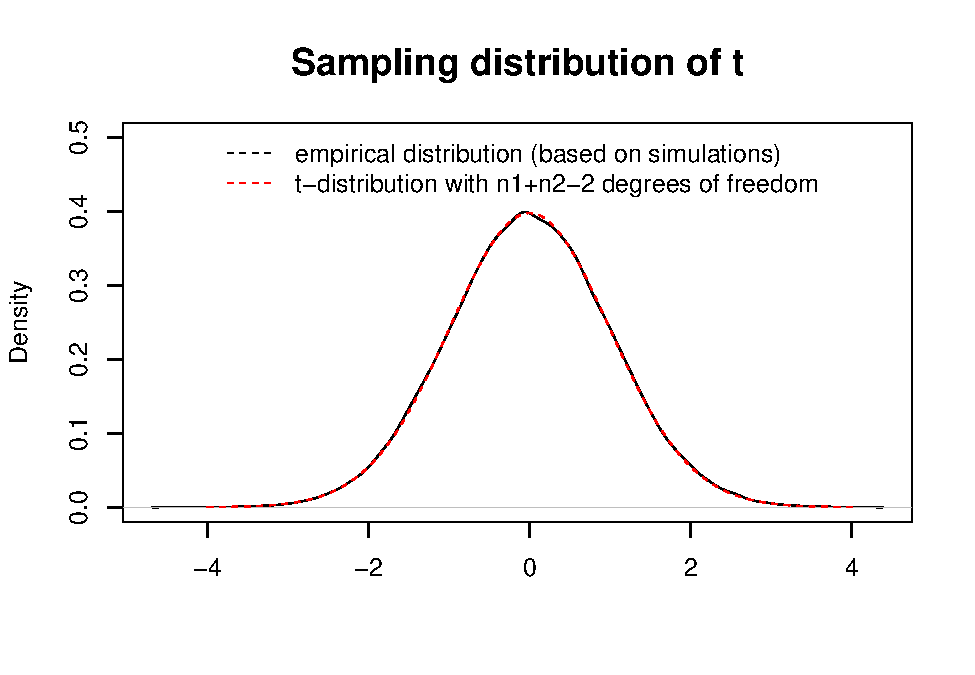
\includegraphics{Appendix2_files/figure-latex/SAMPLMEANDIFF1-1.pdf}
\caption{\label{fig:SAMPLMEANDIFF1}Sampling distribution of Student's t under the assumptions of normality and homoscedasticity}
\end{figure}

Under the null hypothesis, this quantity will follow a central \emph{t}- distribution with \(n_1+n_2-2\) degrees of freedom (see Figure \ref{fig:SAMPLMEANDIFF1}) \footnote{Distribution is central because under the null hypothesis, the quantity is a (supposed normal) centered variable, divided by SE, an independant variable closely related with the $\chi^2$}. We can therefore easily define \((\mu_1-\mu_2)_L\), the lower limit of the confidence interval, such as \(\frac{(\bar{X_1}-\bar{X_2})-(\mu_1-\mu_2)_L}{SE}\) exactly equals the quantile (1-\(\frac{\alpha}{2}\)) of the central \emph{t}-distribution of the null hypothesis \(H_0: \mu_1 - \mu_2 = (\mu_1-\mu_2)_L\), and the upper limit \((\mu_1-\mu_2)_U\) such as \(\frac{(\bar{X_1}-\bar{X_2})-(\mu_1-\mu_2)_U}{SE}\) exactly equals the quantile \(\frac{\alpha}{2}\) of the central \emph{t}-distribution of the null hypothesis \(H_0: \mu_1 - \mu_2 = (\mu_1-\mu_2)_U\):

\begin{equation} 
Pr[t_{n_1+n_2-2} \geq \frac{(\bar{X_1}-\bar{X_2})-(\mu_1-\mu_2)_L}{SE}]= \frac{\alpha}{2}
\label{eq:plausiblelimit1}
\end{equation}

\begin{equation} 
Pr[t_{n_1+n_2-2} \leq \frac{(\bar{X_1}-\bar{X_2})-(\mu_1-\mu_2)_U}{SE}]= \frac{\alpha}{2}
\label{eq:plausiblelimit2}
\end{equation}

\begin{figure}
\centering
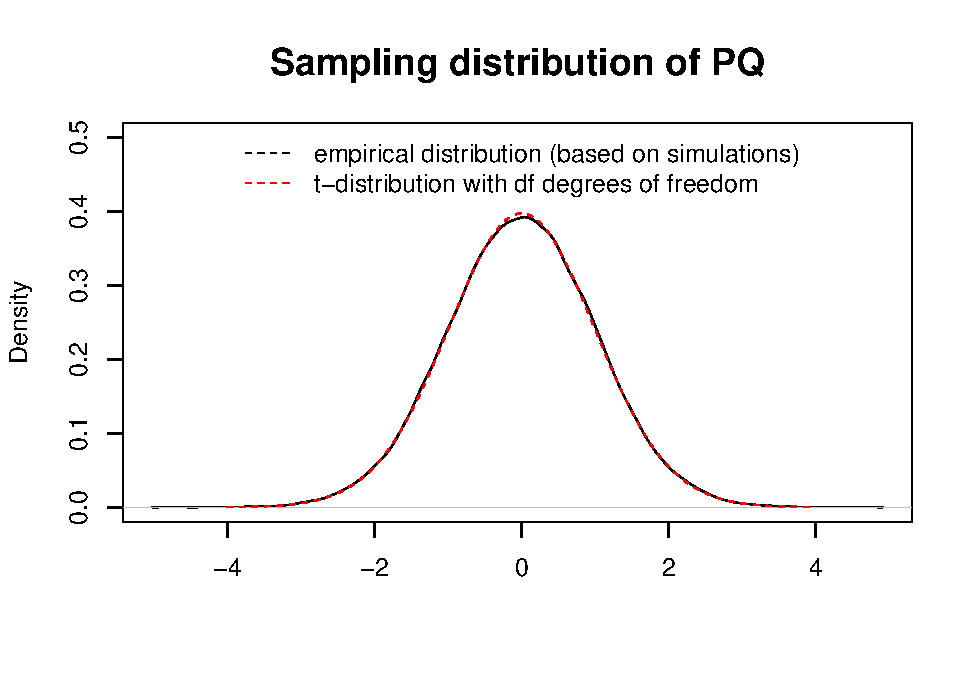
\includegraphics{Appendix2_files/figure-latex/SAMPLMEANDIFF2-1.pdf}
\caption{\label{fig:SAMPLMEANDIFF2}Sampling distribution of Welch's t under the assumptions of normality and heteroscedasticity}
\end{figure}

Under the assumption of iid normal distributions of residuals with unequal variances across groups, in order to test the null hypothesis that \(\mu_1-\mu_2= (\mu_1-\mu_2)_0\), we can compute the following quantity:

\begin{equation} 
t_{Welch}=\frac{(\bar{X_1}-\bar{X_2})-(\mu_1-\mu_2)_0}{SE}
\label{eq:twelch}
\end{equation}

With \(SE = \sqrt{\frac{S^2_1}{n1}+\frac{S^2_2}{n2}}\). Again, under the null hypothesis, we know that this quantity will follow a central \emph{t}- distribution with \(DF=\frac{(\frac{S^2_1}{n_1}+\frac{S^2_2}{n_2})^2}{\frac{(\frac{S^2_1}{n_1})^2}{n_1-1}+\frac{(\frac{S^2_2}{n_2})^2}{n_2-1}}\) degrees of freedom. (see Figure \ref{fig:SAMPLMEANDIFF2}). We can therefore easily define \((\mu_1-\mu_2)_L\) such as \(\frac{(\bar{X_1}-\bar{X_2})-(\mu_1-\mu_2)_L}{SE}\) exactly equals the quantile (1-\(\frac{\alpha}{2}\)) of the central \emph{t}-distribution of the null hypothesis \(H_0: \mu_1 - \mu_2 = (\mu_1-\mu_2)_L\), and the upper limit \((\mu_1-\mu_2)_U\) such as \(\frac{(\bar{X_1}-\bar{X_2})-(\mu_1-\mu_2)_U}{SE}\) exactly equals the quantile \(\frac{\alpha}{2}\) of the central \emph{t}-distribution of the null hypothesis \(H_0: \mu_1 - \mu_2 = (\mu_1-\mu_2)_U\):

\begin{equation} 
Pr[t_{DF} \geq \frac{(\bar{X_1}-\bar{X_2})-(\mu_1-\mu_2)_L}{SE}]= \frac{\alpha}{2}
\label{eq:plausiblelimit1}
\end{equation}

\begin{equation} 
Pr[t_{DF} \leq \frac{(\bar{X_1}-\bar{X_2})-(\mu_1-\mu_2)_U}{SE}]= \frac{\alpha}{2}
\label{eq:plausiblelimit2}
\end{equation}

It is not the most conventional way of computing confidences limits around any mean differences, but this approach is interesting as it helps to understand how to compute confidence limits around a measure of effect size.

\hypertarget{how-to-compute-a-confidence-interval-around-cohens-delta}{%
\subsubsection{\texorpdfstring{How to compute a confidence interval around Cohen's \(\delta\)}{How to compute a confidence interval around Cohen's \textbackslash delta}}\label{how-to-compute-a-confidence-interval-around-cohens-delta}}

\begin{figure}
\centering
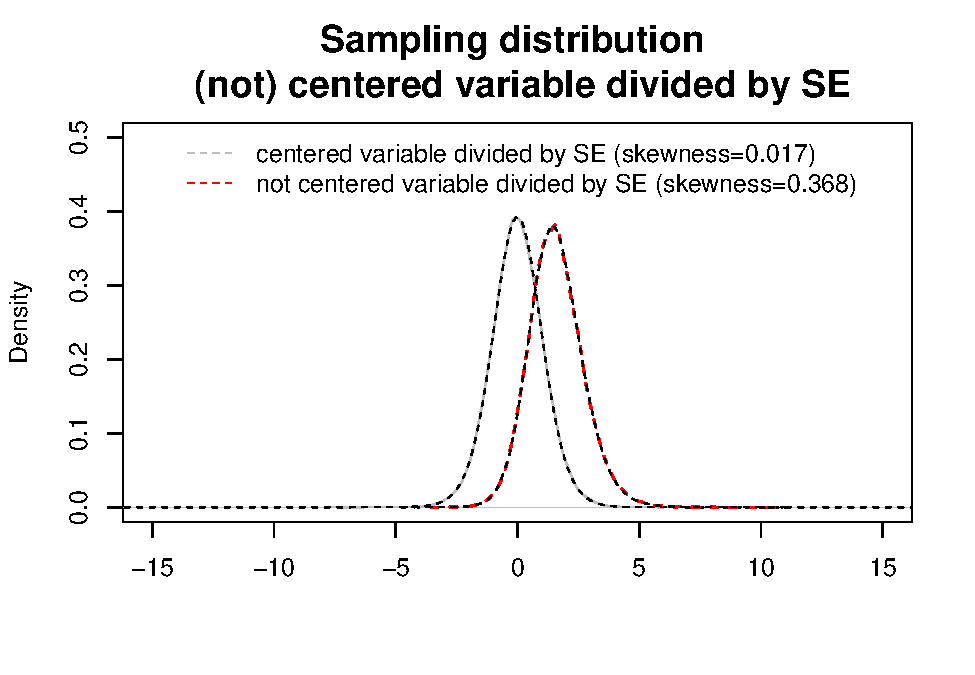
\includegraphics{Appendix2_files/figure-latex/SAMPLMEANDIFF3-1.pdf}
\caption{\label{fig:SAMPLMEANDIFF3}Sampling distribution of centered mean difference divided by SE (in grey, i.e.~pivotal quantity) and not centered mean difference divided by SE (in red), assuming normality and homoscedasticity.}
\end{figure}

We previously mentioned that if the null hypothesis is true,\(t_{Student}\) (see equation \eqref{eq:tstudent}) will follow a central \emph{t}-distribution. However, if the null hypothesis is false, the distribution of this quantity will not be centered, and noncentral \emph{t}-distribution will arise ({\textbf{???}}), as illustrated in Figure \ref{fig:SAMPLMEANDIFF3}.

Noncentral \emph{t}-distributions are described by two parameters: degrees of freedom (df) and noncentrality parameter (that we will call \(\Delta\); {\textbf{???}}), the last being a function of \(\delta\) and sample sizes \(n_1\) and \(n_2\):

\begin{equation}
\Delta = \frac{\mu_1-\mu_2}{\sigma_{pooled}} \times \sqrt{\frac{n_1 \times n_2}{n_1 + n_2}}
\label{eq:ncp}
\end{equation}

Considering the link between \(\Delta\) and \(\delta\), it is possible to compute confidence limits for \(\Delta\), and divide them by \(\sqrt{\frac{n_1 \times n_2}{n_1 + n_2}}\) in order to have confidence limits for \(\delta\). In other word, we first need to determine the noncentrality parameters of the \emph{t}-distributions for which \(t_{Student}\) corresponds respectively to the \(1-\frac{\alpha}{2}\) and to the \(\frac{\alpha}{2}\) th. quantile:

\[P[t_{df, \Delta_L} \geq t_{Student}] = \frac{\alpha}{2} \]

\[P[t_{df, \Delta_U} \leq t_{Student}] = \frac{\alpha}{2} \]

With \(df = n_1+n_2-2\). Second, we divide \(\Delta_L\) and \(\Delta_U\) by \(\sqrt{\frac{n_1 \times n_2}{n_1 + n_2}}\) in order to define \(\delta_L\) and \(\delta_U\):

\[\delta_L = \frac{\Delta_L}{\sqrt{\frac{n_1 \times n_2}{n_1 + n_2}}}\]

\[\delta_U = \frac{\Delta_U}{\sqrt{\frac{n_1 \times n_2}{n_1 + n_2}}}\]

\hypertarget{how-to-determine-the-confidence-interval-around-shiehs-delta}{%
\section{\texorpdfstring{How to determine the confidence interval around Shieh's \(\delta*\)}{How to determine the confidence interval around Shieh's \textbackslash delta*}}\label{how-to-determine-the-confidence-interval-around-shiehs-delta}}

Like \(t_{Student}\), \(t_{Welch}\) (see equation \eqref{eq:twelch}) will follow a central \emph{t}-distribution only if the null hypothesis is true. If the null hypothesis is false, it will follow a noncentral \emph{t}-distribution, as illustrated in Figure \ref{fig:SAMPLMEANDIFF4}.

\begin{figure}
\centering
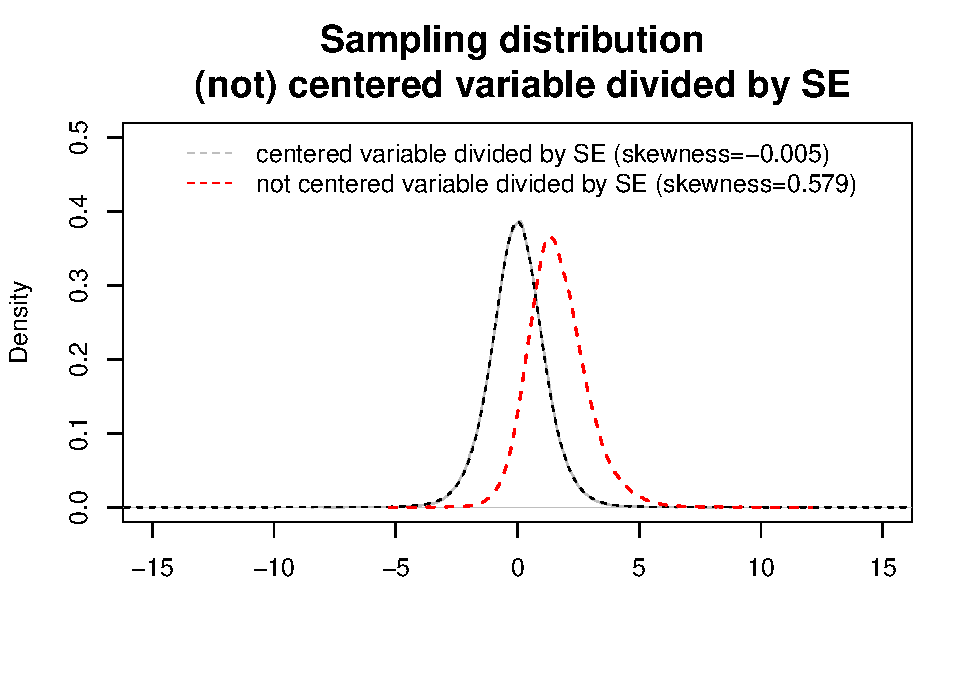
\includegraphics{Appendix2_files/figure-latex/SAMPLMEANDIFF4-1.pdf}
\caption{\label{fig:SAMPLMEANDIFF4}Sampling distribution of centered mean difference divided by SE (in grey, i.e.~pivotal quantity) and not centered mean difference divided by SE (in red), assuming normality and homoscedasticity.}
\end{figure}

The noncentrality parameter \(\Delta*\) is a function of \(\delta*\) and total sample size \(N = n_1 + n_2\) ({\textbf{???}})

\begin{equation}
\Delta* = \frac{\mu_1-\mu_2}{\sqrt{\frac{\sigma_1^2}{n_1/N}+\frac{\sigma_2^2}{n_2/N}}} \times \sqrt{N}
\label{eq:ncp}
\end{equation}

Considering the link between \(\Delta\) and \(\delta\), we can compute confidence limits for \(\Delta*\), and divide them by \(\sqrt{N}\) in order to have confidence limits for \(\delta*\). We first need to determine the noncentrality parameters of the distributions for which \(t_{Welch}\) corresponds respectively to the \(1-\frac{\alpha}{2}\) and to the \(\frac{\alpha}{2}\) th. quantile.
\[P[t_{v, \Delta*_L} \geq t_{Welch}] = \frac{\alpha}{2} \] and
\[P[t_{v, \Delta*_U} \leq t_{Welch}] = \frac{\alpha}{2} \].

With \emph{v} approximated by \(\hat{v} = \frac{(\frac{S_1^2}{n_1}+\frac{S_2^2}{n_2})^2}{\frac{(\frac{S_1^2}{n_1})^2}{n_1-1}+\frac{(\frac{S_2^2}{n_2})^2}{n_2-1}}\) ({\textbf{???}})

Second, we divide \(\Delta*_L\) and \(\Delta*_U\) by \(\sqrt{N}\) in order to have \(\delta*_L\) and \(\delta*_U\) (i.e.~confidences limits for Shieh's \(\delta*\)).

\end{document}
